\subsection{Pruebas Preliminares.}
\label{chap:pruebas preliminares}
\subsubsection{Par\'ametros de control.}

A manera de control, 2 de las corridas preliminares se realizaron empleando los par\'ametros correspondientes a rocas sanas, es decir a la arenisca de la FM. Pottsville y Limolita de la Fm. Repetto. Los DEM resultantes se muestran en las figuras \ref{fig:pottsville} y \ref{fig:repetto}.
Asimismo, entre los archivos de texto producto de ambas corridas, espec\'ificamente el archivo \_out.txt. se puede observar\linebreak


\pagebreak
\begin{center}
\textbf{siltySand\_12\_38\_27\_out.txt}

\begin{verbatim}
3D POTENTIAL FAILURE - GLOBAL MINIMUM
Bishop's 3D factor of safety:                                          15.1517
Ordinary 3D factor of safety:                                          15.1517
Volume (m ^3):                                                     3.33350E+04
Horizontal surface area (m ^2):                                    5.78697E+03
Slip surface area (m ^2):                                          5.80648E+03
Weight (kg):                                                       8.66710E+05
\end{verbatim}
\end{center}

\begin{center}

\textbf{34\_32\_23\_out.txt}
\begin{verbatim}
3D POTENTIAL FAILURE - GLOBAL MINIMUM
Bishop's 3D factor of safety:                                          12.2276
Ordinary 3D factor of safety:                                          12.2276
Volume (m ^3):                                                     3.33350E+04
Horizontal surface area (m ^2):                                    5.78697E+03
Slip surface area (m ^2):                                          5.80648E+03
Weight (kg):                                                       7.66705E+05
\end{verbatim}

\end{center}
N\'otese adem\'as que los factores de seguridad m\'iinimos son 15.15 y 12.22 para los ensayos realizados con los par\'ametros de la Fm. Repetto y Fm. Pottsville respectivamente, y las masas de material removido son de $8.66^{5}$ Kg y $7.66^{5}$Kg

\subsubsection{Par\'ametros de prueba: Fm. Bukit Timah.}
\begin{figure}[H]
\centering
\begin{minipage}{.45\linewidth}
  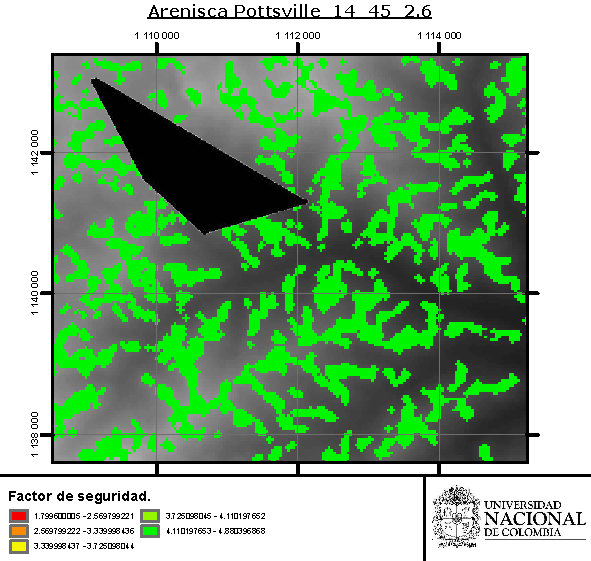
\includegraphics[width=\linewidth]{AreniscaPottsville.pdf}
  \captionof{figure}{Simulaci\'on con par\'ametros tomado de la arenisca de Fm. Pottsville.}
  \label{fig:pottsville}
\end{minipage}
\hspace{.05\linewidth}
\begin{minipage}{.45\linewidth}
  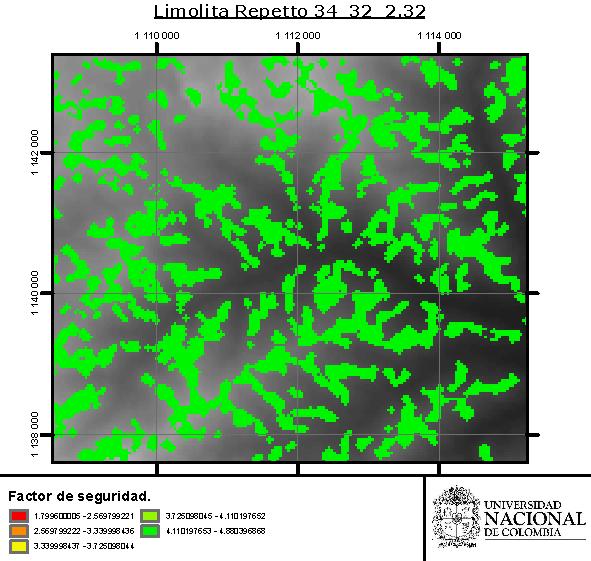
\includegraphics[width=\linewidth]{img/LimolitaRepetto34_32_232.pdf}
  \captionof{figure}{Simulaci\'on con par\'ametros tomado de la limolita de Fm. Repetto.}
  \label{fig:repetto}
\end{minipage}
\end{figure}

Al usar los par\'metros correspondientes a los distintos niveles de meteorizaci\'on de la formaci\'on Bukit Timah, se puede apreciar que a medida que se incrementa el nivel de clasificaci\'on, mayores extensiones de \'area muestran reducci\'on en el factor de seguridad.
Se aprecia igualmente que los fondos de los valles as\'i como los filos de las laderas no exhiben ocurrencia de superficies de falla, ello debido a la disminuci\'on en las pendientes existentes, aun cuando se ha buscado centros de esfera a alturas superiores a los 17.000 msnm.


\subsubsection{Par\'ametros de prueba: Fm. Jurong.}

\begin{figure}[H]
\centering
\begin{minipage}{.45\linewidth}
  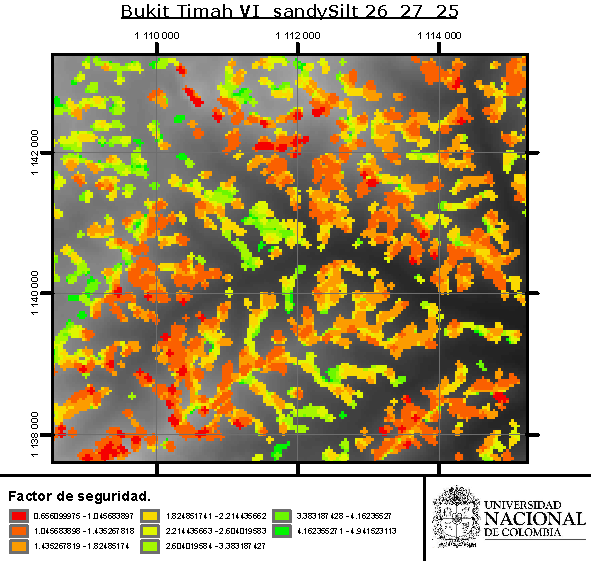
\includegraphics[width=\linewidth]{Bukit_Timah_VI_sandySilt_26_27_25.pdf}
  \captionof{figure}{}
  \label{fig:bukit1}
\end{minipage}
\hspace{.05\linewidth}
\begin{minipage}{.45\linewidth}
  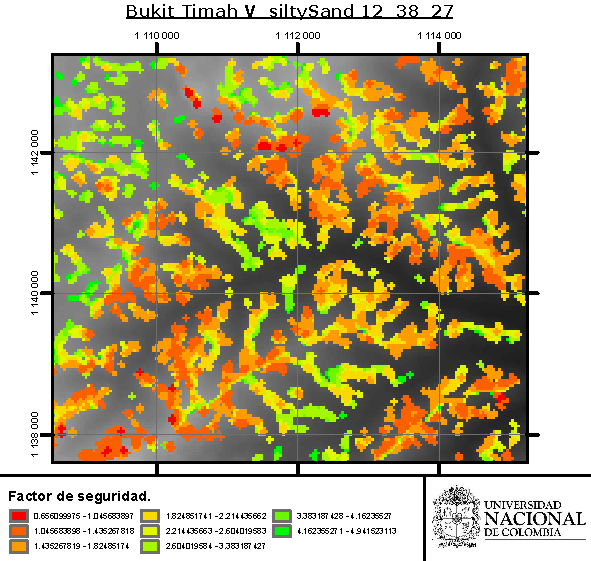
\includegraphics[width=\linewidth]{Bukit_Timah_V_siltySand_12_38_27.pdf}
  \captionof{figure}{}
  \label{fig:bukit2}
\end{minipage}
\begin{minipage}{.45\linewidth}
  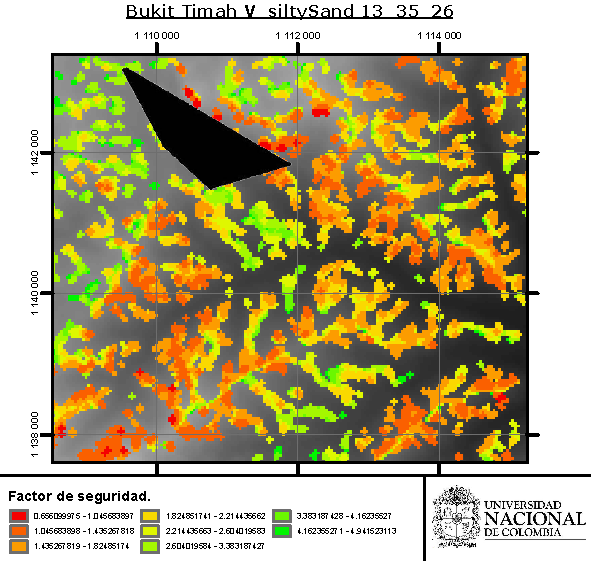
\includegraphics[width=\linewidth]{BukitTimahV_siltySand13_35_26.pdf}
  \captionof{figure}{}
  \label{fig:bukit3}
\end{minipage}
\end{figure}




Simulaciones con Par\'metros de la Fm. Jurong.


\begin{figure}[H]
\centering
\begin{minipage}{.45\linewidth}
  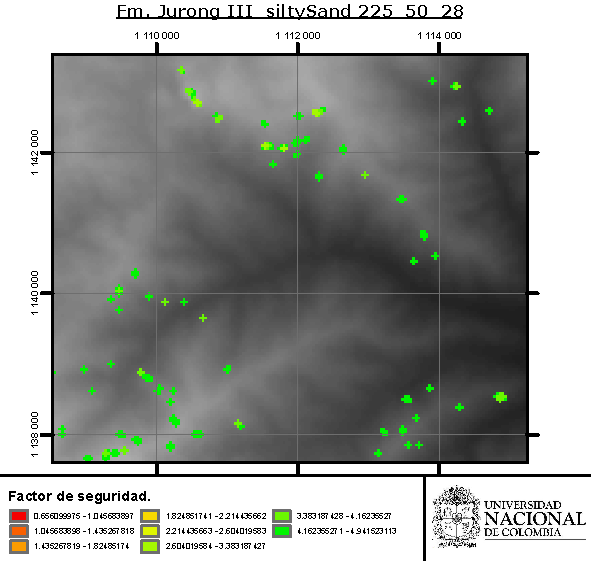
\includegraphics[width=\linewidth]{Fm_JurongIII_siltySand225_50_28.pdf}
  \captionof{figure}{}
  \label{fig:jurong1}
\end{minipage}
\hspace{.05\linewidth}
\begin{minipage}{.45\linewidth}
  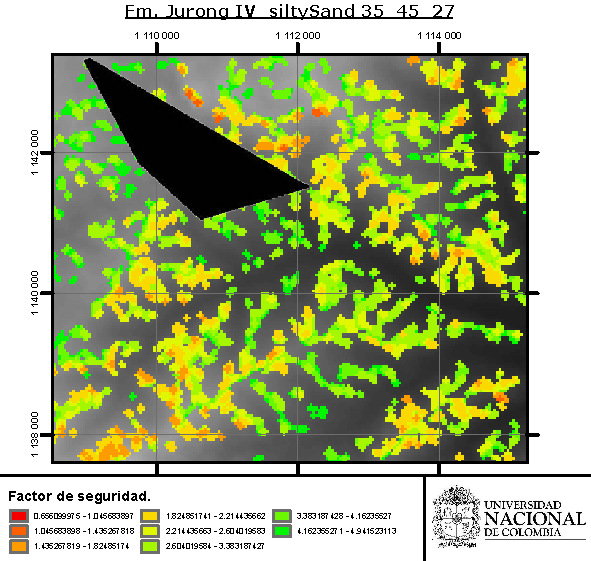
\includegraphics[width=\linewidth]{Fm_JurongIV_siltySand35_45_27.pdf}
  \captionof{figure}{}
  \label{fig:jurong2}
\end{minipage}
\begin{minipage}{.45\linewidth}
  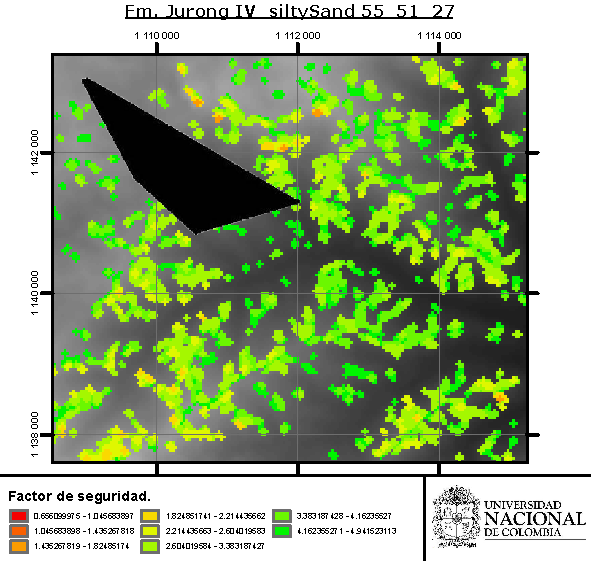
\includegraphics[width=\linewidth]{Fm_JurongIV_siltySand55_51_27.pdf}
  \captionof{figure}{}
  \label{fig:jurong3}
\end{minipage}
\begin{minipage}{.45\linewidth}
  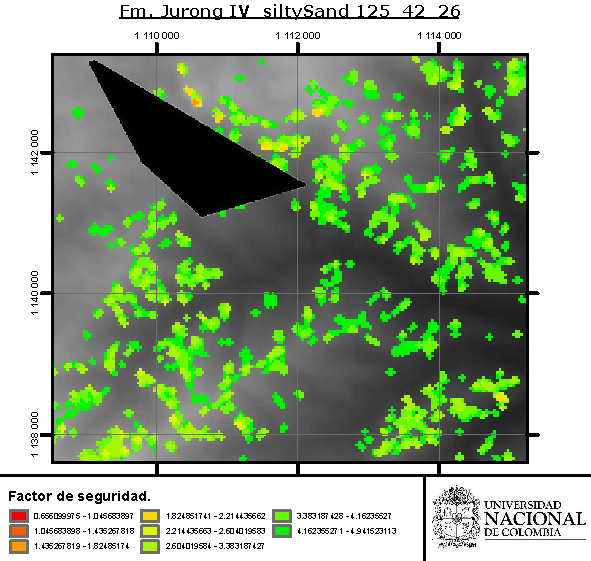
\includegraphics[width=\linewidth]{Fm_JurongIV_siltySand125_42_26.pdf}
  \captionof{figure}{}
  \label{fig:jurong4}
\end{minipage}
\end{figure}


Se puede apreciar que en las pruebas realizadas con par\'ametros correspondientes a muestras m\'s superficiales, la dispersi\'on de colores rojizos y anaranjados es mas predominante sobre la zona  de trabajo. Ello indicando una disminuci\'on en los factores de seguridad en las laderas de la zona de estudio.\par

\subsection{Interpretacion}
Es posible es posible apreciar, basado en los resultados obtenidos en la Subsecci\'on \ref{chap:pruebas preliminares} que debido a la alta variabilidad de pendientes que se presentan en la zona de trabajo, las cuales var\'ian desde bajas hasta altas y muy altas, sumado a la importante longitud de las laderas . Que el rango de factores de seguridad obtenidos con el software Scoops3D var\'ia desde valores inferiores a 1 que implican falla, hasta valores que tienen como resultado factores de seguridad superiores a 5.
Es importante tener en cuenta que esta simulaci\'on no contempla factores externos como la sobrecarga de la cobertura vegetal ni la actividad antr\'opica, que se da fuertemente en la zona y cuya presencia puede implicar la existencia en la zona de agentes qu\'imicos que debiliten la agregaci\'on de particulas y contribuya en una potencial disminuci\'on de la cohesi\'on de los materiales.

Asimismo se puede apreciar que a medida que las pruebas realizadas con materiales que indican un estado mas avanzado del proceso de meteorizaci\'on, y por ende poseen una mayor proporci\'on de fraccion arcillosa y \'oxidos e hidr\'oxidos de hierro y aluminio, tienen como resultado una marcada disminuci\'on en los factores de seguridad. Tal como se puede apreciar al compararlas im\'agenes XXX y XXX de las pruebas realizadas con los parámetros de resistencia de la Fm. Jurong.

Basado en el origen y tipo de materiales presentes en la cuenca hidrogr\'afica de la Qda.La Linda, se esperaria que los parametros de resistencia hayados en campo se aproximen considerablemente a los usados para la simulacion ilustrada en las figuras \ref{fig:jurong2} o \ref{fig:jurong3}. Es de esperarse en 

